\documentclass[12pt,a4paper,parskip=full]{scrartcl}
\usepackage{float}
% \usepackage{bbding}
% \usepackage{pifont}
% \usepackage{wasysym}
\usepackage[default,scale=1]{opensans} 
%\usepackage[T1]{fontenc}
\usepackage[margin=1in]{geometry}
\geometry{letterpaper}
\usepackage{xcolor}
\definecolor{red}{HTML}{cc0000}
\definecolor{gray}{HTML}{666666}
\usepackage{sectsty}
\sectionfont{\color{red}}
\subsectionfont{\fontsize{25}{25}\color{red}}
\subsubsectionfont{\fontsize{20}{20}\color{red}}
\usepackage{graphicx}
\usepackage{hyperref}
%\usepackage{amssymb}
\usepackage[style=footnote-dw]{biblatex}
\bibliography{S@SGuideBib}
\setlength\bibitemsep{0.5\baselineskip}
\graphicspath{{./images/}}

\usepackage{enumitem}
%\setitemize{noitemsep}
% \setlist{noitemsep, topsep=-5pt}
% \setlength\itemsep{-0.10em}

\renewcommand{\labelitemi}{$\cdot$}
\renewcommand{\labelitemii}{$\cdot$}
\makeatletter
\let\latexl@section\l@section
\def\l@section#1#2{\begingroup\let\numberline\@gobble\latexl@section{#1}{#2}\endgroup}
\makeatother

\usepackage[T1]{fontenc}
\fontfamily{verdana}

%\usepackage{scrlayer-scrpage}{}
\usepackage{fancyhdr}
\makeatletter
\renewcommand{\@seccntformat}[1]{}
\makeatother

\setlength\parindent{0pt}{}

\pagestyle{fancy}
\fancyhf{}
\lhead{ \fancyplain{}{The Scrum@Scale Guide}}
\rfoot{ \fancyplain{}{\thepage} }
\lfoot{\textcopyright 2006-2021 Jeff Sutherland \& Scrum Inc.}



\title{\Huge{\color{red}\textbf{The Scrum@Scale 
\textsuperscript{\registered} 
Guide}}}
\subtitle{\color{gray}The Definitive Guide to Scrum@Scale:\\ Scaling that Works}
% \author{}
\date{}




\begin{document}
\tableofcontents

\subsection{Preface to the Scrum@Scale
Guide}\label{preface-to-the-ScrumatScale-guide}

Scrum, as originally outlined in the Scrum Guide, is focused on a single Scrum Team being able to deliver optimal value while maintaining a sustainable pace. Since its inception, the usage of Scrum has extended to the creation of products, processes, and services that require the efforts of multiple teams. 

In the field, it was repeatedly observed that as the number of Scrum Teams within an organization grew, two major issues emerged:


\begin{itemize}%[label={\huge\textbullet}]
\itemsep10pt
\item
  The volume, speed, and quality of their output (working product) per team began to fall, due to issues such as cross-team dependencies, duplication of work, and communication overhead 
\item
 The original management structure was ineffective for achieving business agility. Issues arose like competing priorities and the inability to quickly shift teams around to respond to dynamic market conditions
\end{itemize}

To counteract these issues, a framework for effectively coordinating multiple Scrum Teams was clearly needed which would aim for the following:

\begin{itemize}
\itemsep10pt
\item
  Linear scalability: A corresponding percentage increase in delivery of working product with an increase in the number of teams
\item
 Business agility: The ability to rapidly respond to change by adapting the initial stable configuration
\end{itemize}

Scrum@Scale helps an organization to focus multiple networks of Scrum Teams on prioritized goals. It aims to achieve this by setting up a structure which naturally extends the way a single Scrum Team functions across a network and whose managerial function exists within a minimum viable bureaucracy (MVB).


A network can achieve linear scalability when its characteristics are independent of its size. Designing and coordinating a network of teams with this goal does not constrain growth in a particular way; instead, it allows for the network to grow organically, based on its unique needs, and at a sustainable pace of change that can be better accepted by the individuals involved. 

A minimum viable bureaucracy is defined as having the least amount of governing bodies and processes needed to carry out the function(s) of an organization without impeding the delivery of customer value. It helps to achieve business agility by reducing decision latency (time to make a decision), which has been noted as a primary driver of success. In order to begin implementing Scrum@Scale, it is essential to be familiar with the Agile Manifesto and the 2020 Scrum Guide. A failure to understand the nature of agility will prevent it from being achieved. If an organization cannot Scrum, it cannot scale.


\subsection{Purpose of the Scrum@Scale
Guide}\label{purpose-of-the-ScrumatScale-guide}

This guide provides the definition of Scrum@Scale and the components of its framework. It explains the accountabilities of the scaled roles, scaled events, and enterprise artifacts, as well as the rules that bind them together.

This guide is broken down into four basic sections:

\begin{itemize}
\itemsep1pt\parskip0pt\parsep0pt
\item
  an introduction to Scrum@Scale, with the basics for getting started
\item
  an overview of the Scrum Master Cycle
\item
  an overview of the Product Owner Cycle
\item
  a walk-through of bringing the cycles together
\end{itemize}

Each component serves a specific purpose which is required for success at scale. Changing their core design or ideas, omitting them, or not following the base rules laid out in this guide limits the benefits of Scrum@Scale.

Specific tactics beyond the basic structure and rules for implementing each component vary and are not described in this Guide. Other sources provide complementary patterns, processes, and insights.

\subsection{Definitions}\label{definitions}

Scrum is a lightweight framework that helps people, teams and organizations generate value through adaptive solutions for complex problems.

The Scrum Guide describes the minimal set of elements that create a team environment that drives innovation, customer satisfaction, performance, and happiness. Scrum utilizes radical transparency and a series of formal events to provide opportunities to inspect and adapt a team and its product(s).

Scrum@Scale is a lightweight organizational framework in which a network of teams operating consistently with the Scrum Guide can address complex adaptive problems, while creatively delivering products of the highest possible value. These ``products'' may be physical, digital, complex integrated systems, processes, services, etc.

The Scrum@Scale Guide describes the minimal set of components to scale Scrum by using Scrum and its resulting business agility across an entire organization. It can be used in all types of organizations within industry, government, nonprofits, or academia. If an organization does not already use Scrum, it will require changes to its operating system.

In Scrum, care is taken to separate accountability of the ``what'' (product) from the ``how'' (process). The same care is taken in Scrum@Scale, so that jurisdiction and accountability are expressly understood. This eliminates wasteful organizational conflict that keep teams from achieving their optimal productivity. Because Scrum@Scale consists of components, it allows an organization to customize their transformation strategy and implementation. It gives an organization the ability to target incrementally prioritized change efforts in the area(s) deemed most valuable or most in need of adaptation and then progress on to others.

Scrum@Scale separates these components into two cycles: the Scrum Master Cycle (the ``how'') and the Product Owner Cycle (the ``what''), intersecting at two components and sharing a third. Taken as a whole, these cycles produce a powerful supporting structure for coordinating the efforts of multiple teams along a single path.

\subsection{The Components of
Scrum@Scale}\label{the-components-of-scrumatscale}
\begin{figure}[H]
    \centering
    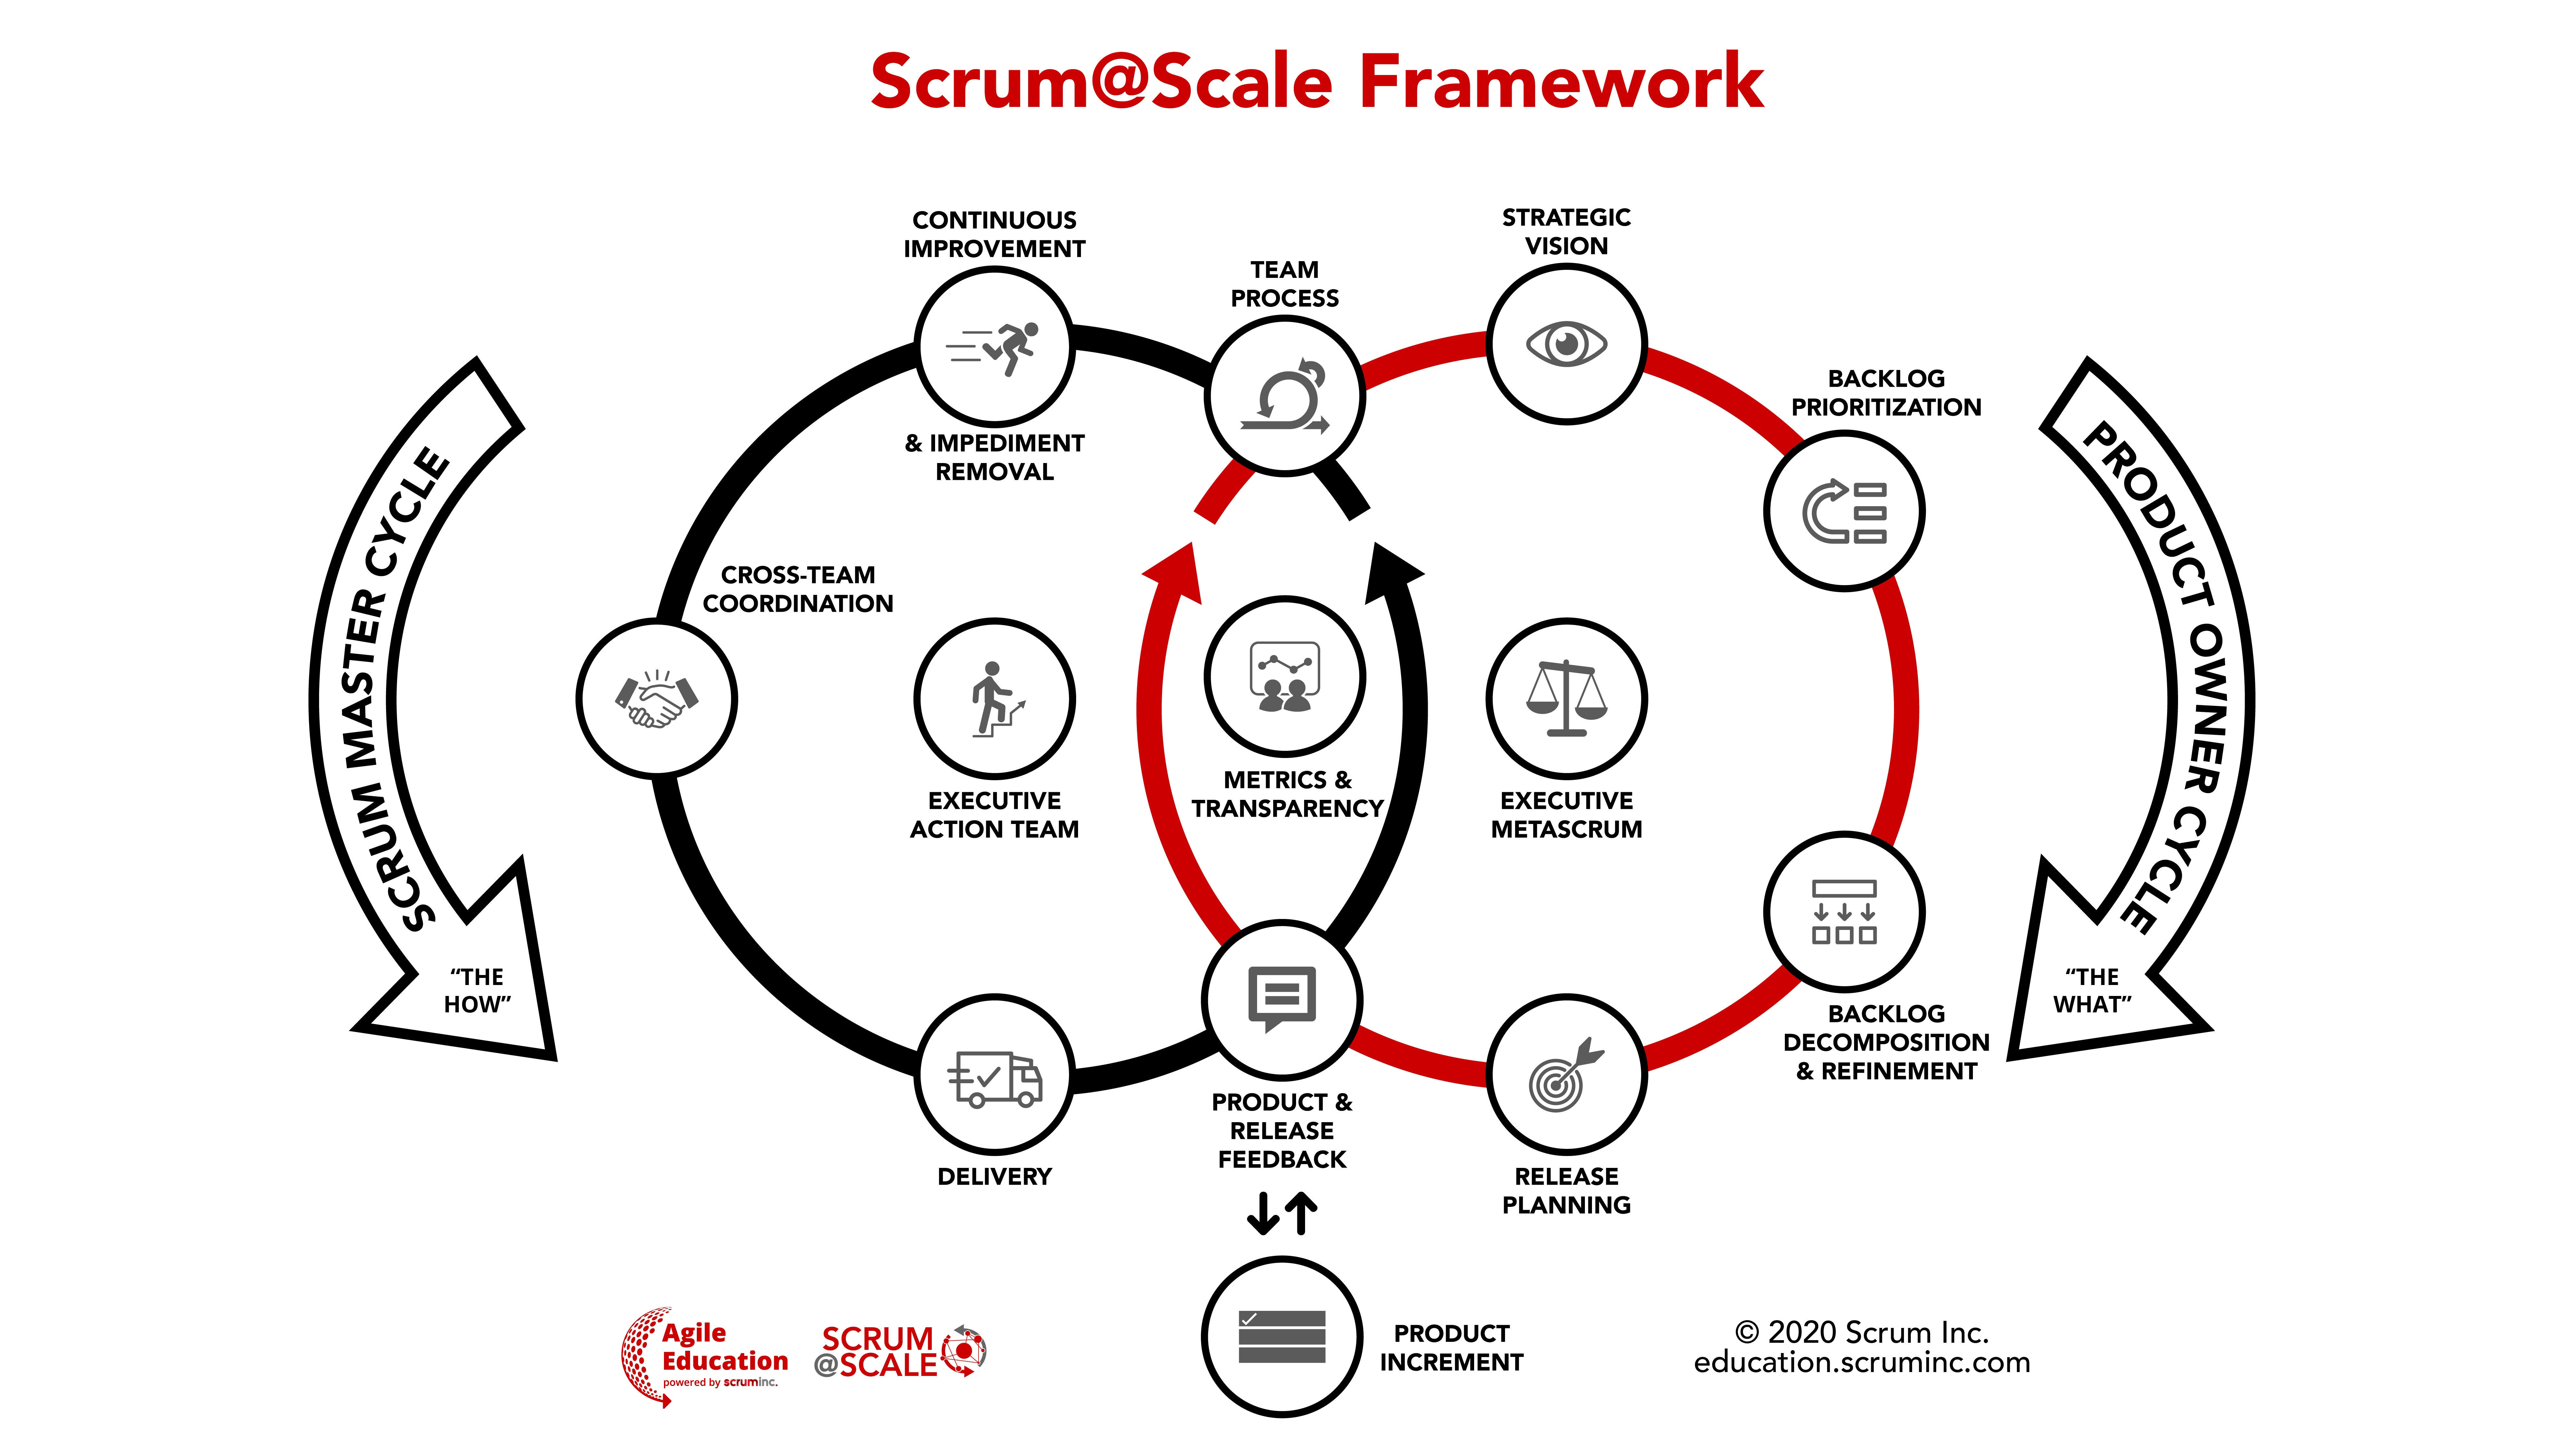
\includegraphics[scale=0.25]{SMPO-Cycle.png}
\end{figure}


\subsubsection{Values-Driven Culture}\label{values-driven-culture}

Scrum@Scale aims to build a healthy organizational culture through the pillars of empirical process control and the Scrum Values. The pillars of empirical process control are transparency, inspection, and adaptation.  These pillars are actualized by the Scrum values of Openness, Courage, Focus, Respect, and Commitment.

Openness supports transparency into all of the work and processes and without it, there is no ability to inspect them honestly and attempt to adapt them for the better. Courage refers to taking the bold leaps required to deliver value quicker in innovative ways. Focus and Commitment refer to the way we handle our work obligations, putting customer value delivery as the highest priority. Lastly, all of this must occur in an environment based on respect for the individuals doing the work, without whom nothing can be created.

Scrum@Scale helps organizations thrive by supporting a positive team learning environment for working at a sustainable pace, while putting customer value at the forefront.


\subsubsection{Getting Started: Installing an Agile Operating
System}\label{getting-started-installing-an-agile-operating-system}

When implementing networks of teams, it is critical to develop a scalable Reference Model prior to scaling. The reference model is a small set of teams that coordinate to deliver every Sprint. As these teams successfully implement Scrum, the rest of the organization has a functioning, healthy example of Scrum to replicate. It serves as a prototype for scaling Scrum across the next network of teams. Any deficiencies in a Scrum implementation will be magnified when multiple teams are deployed. Scaling problems include organizational policies and procedures or development practices that block performance and frustrate teams.

In a scaled setting, the Reference Model is best enabled by grouping teams together that need to coordinate in order to deliver a fully integrated set of Increments into a Scrum of Scrums (SoS). To operate effectively, the Scrum of Scrums needs to be supported by a minimum viable bureaucracy composed of two leadership groups: an Executive MetaScrum (EMS) forum, focused on what is produced by the Scrum of Scrums and an Executive Action Team (EAT) focused on how they can get it done faster. The Executive MetaScrum and Executive Action Team components are the hubs around which each cycle revolves.

\subsubsection{Scaling The Teams}\label{scaling-the-teams}

In Scrum, the ideal state is for a Scrum Team to be an independent path to production. As such, it needs members who have all the skills necessary to go from ideation to implementation. The Scrum of Scrums is a larger team of multiple teams that replicates this ideal at scale. Each team within the Scrum of Scrums must satisfy the Team Process component.

\subsubsection{The Team Process}\label{the-team-process}

The Team Process is Scrum as prescribed by the Scrum Guide. Since every Scrum Team has a Product Owner and a Scrum Master, it constitutes the first intersection between the Product Owner and Scrum Master Cycles. The goals of the Team Process are to:
\begin{itemize}
\itemsep1pt\parskip0pt\parsep0pt
\item
 Maximize the flow of completed work that meets the Definition of Done
\item
  Increase performance of the team over time
\item
  Operate in a way that is sustainable and enriching for the team
\item
  Accelerate the customer feedback loop
\end{itemize}

\subsubsection{The Scrum of Scrums (SoS)}\label{the-scrum-of-scrums}

A Scrum of Scrums operates as if it were a Scrum Team, satisfying the Team Process component with scaled versions of the Scrum accountabilities, events, and artifacts. While the Scrum Guide defines the optimal team size as being fewer than 10 people, Harvard research\textsuperscript{\hyperref[citation4]{4}}  has determined that optimal team size is 4.6 people (on average). Therefore, the optimal number of teams in a Scrum of Scrums is 4 or 5.

As a dynamic group, the teams composing the Scrum of Scrums are responsible for a fully integrated set of potentially shippable increments of product at the end of every Sprint. Optimally, they carry out all of the functions required to release value directly to customers.


\begin{figure}[H]
    \centering
    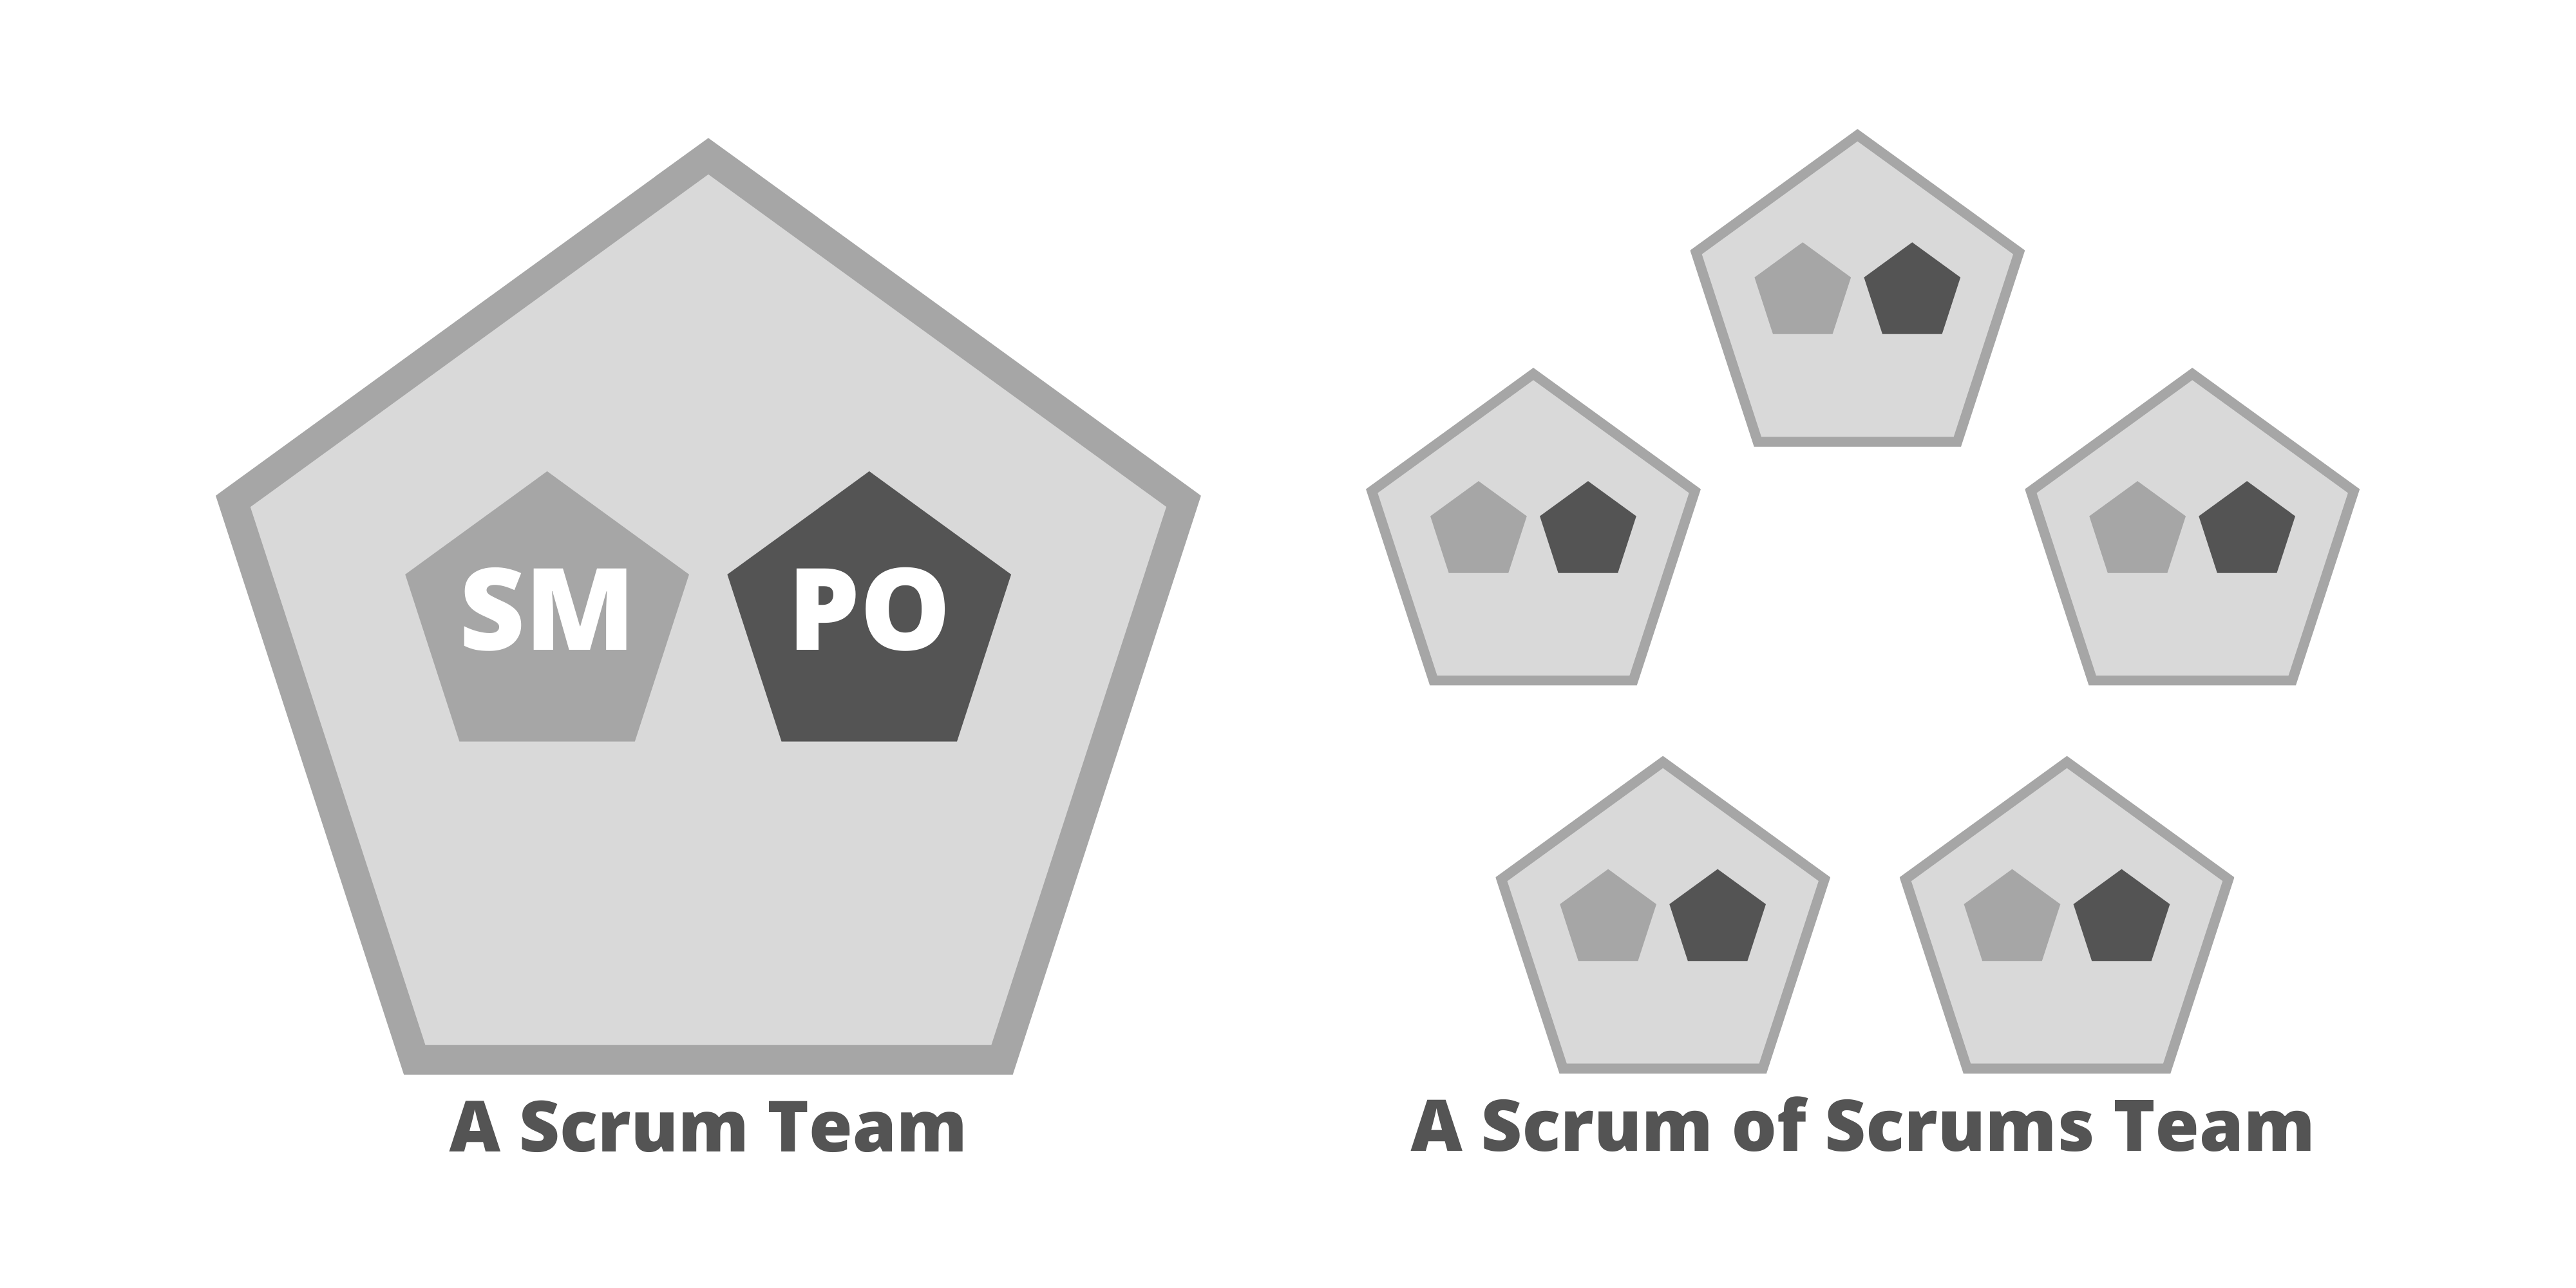
\includegraphics[scale=0.15]{1.png}
\end{figure}


\emph{
 NOTE: In the above and following diagrams, light-grey outlined pentagons represent a team. Where applicable, we have chosen to represent the SM \& PO as smaller pentagons. These diagrams are meant to be examples only, as each organizational diagram may differ greatly.}

\subsubsection{Scaling in Larger
Organizations}\label{scaling-in-larger-organizations}

Depending upon the size of an implementation, more than one Scrum of
Scrums may be needed to deliver a complex product. In such cases, a
Scrum of Scrum of Scrums (SoSoS) can be created out of multiple Scrums
of Scrums. Each of these will have scaled versions of each Scrum of
Scrums' roles, artifacts, and events.

Scaling the Scrum of Scrums reduces the number of communication pathways
within the organization so that complexity of communication overhead is
limited. The SoSoS interfaces with a Scrum of Scrums in the exact same
manner that a Scrum of Scrums interfaces with a single Scrum Team, which
allows for linear scalability.

\begin{figure}[H]
    \centering
    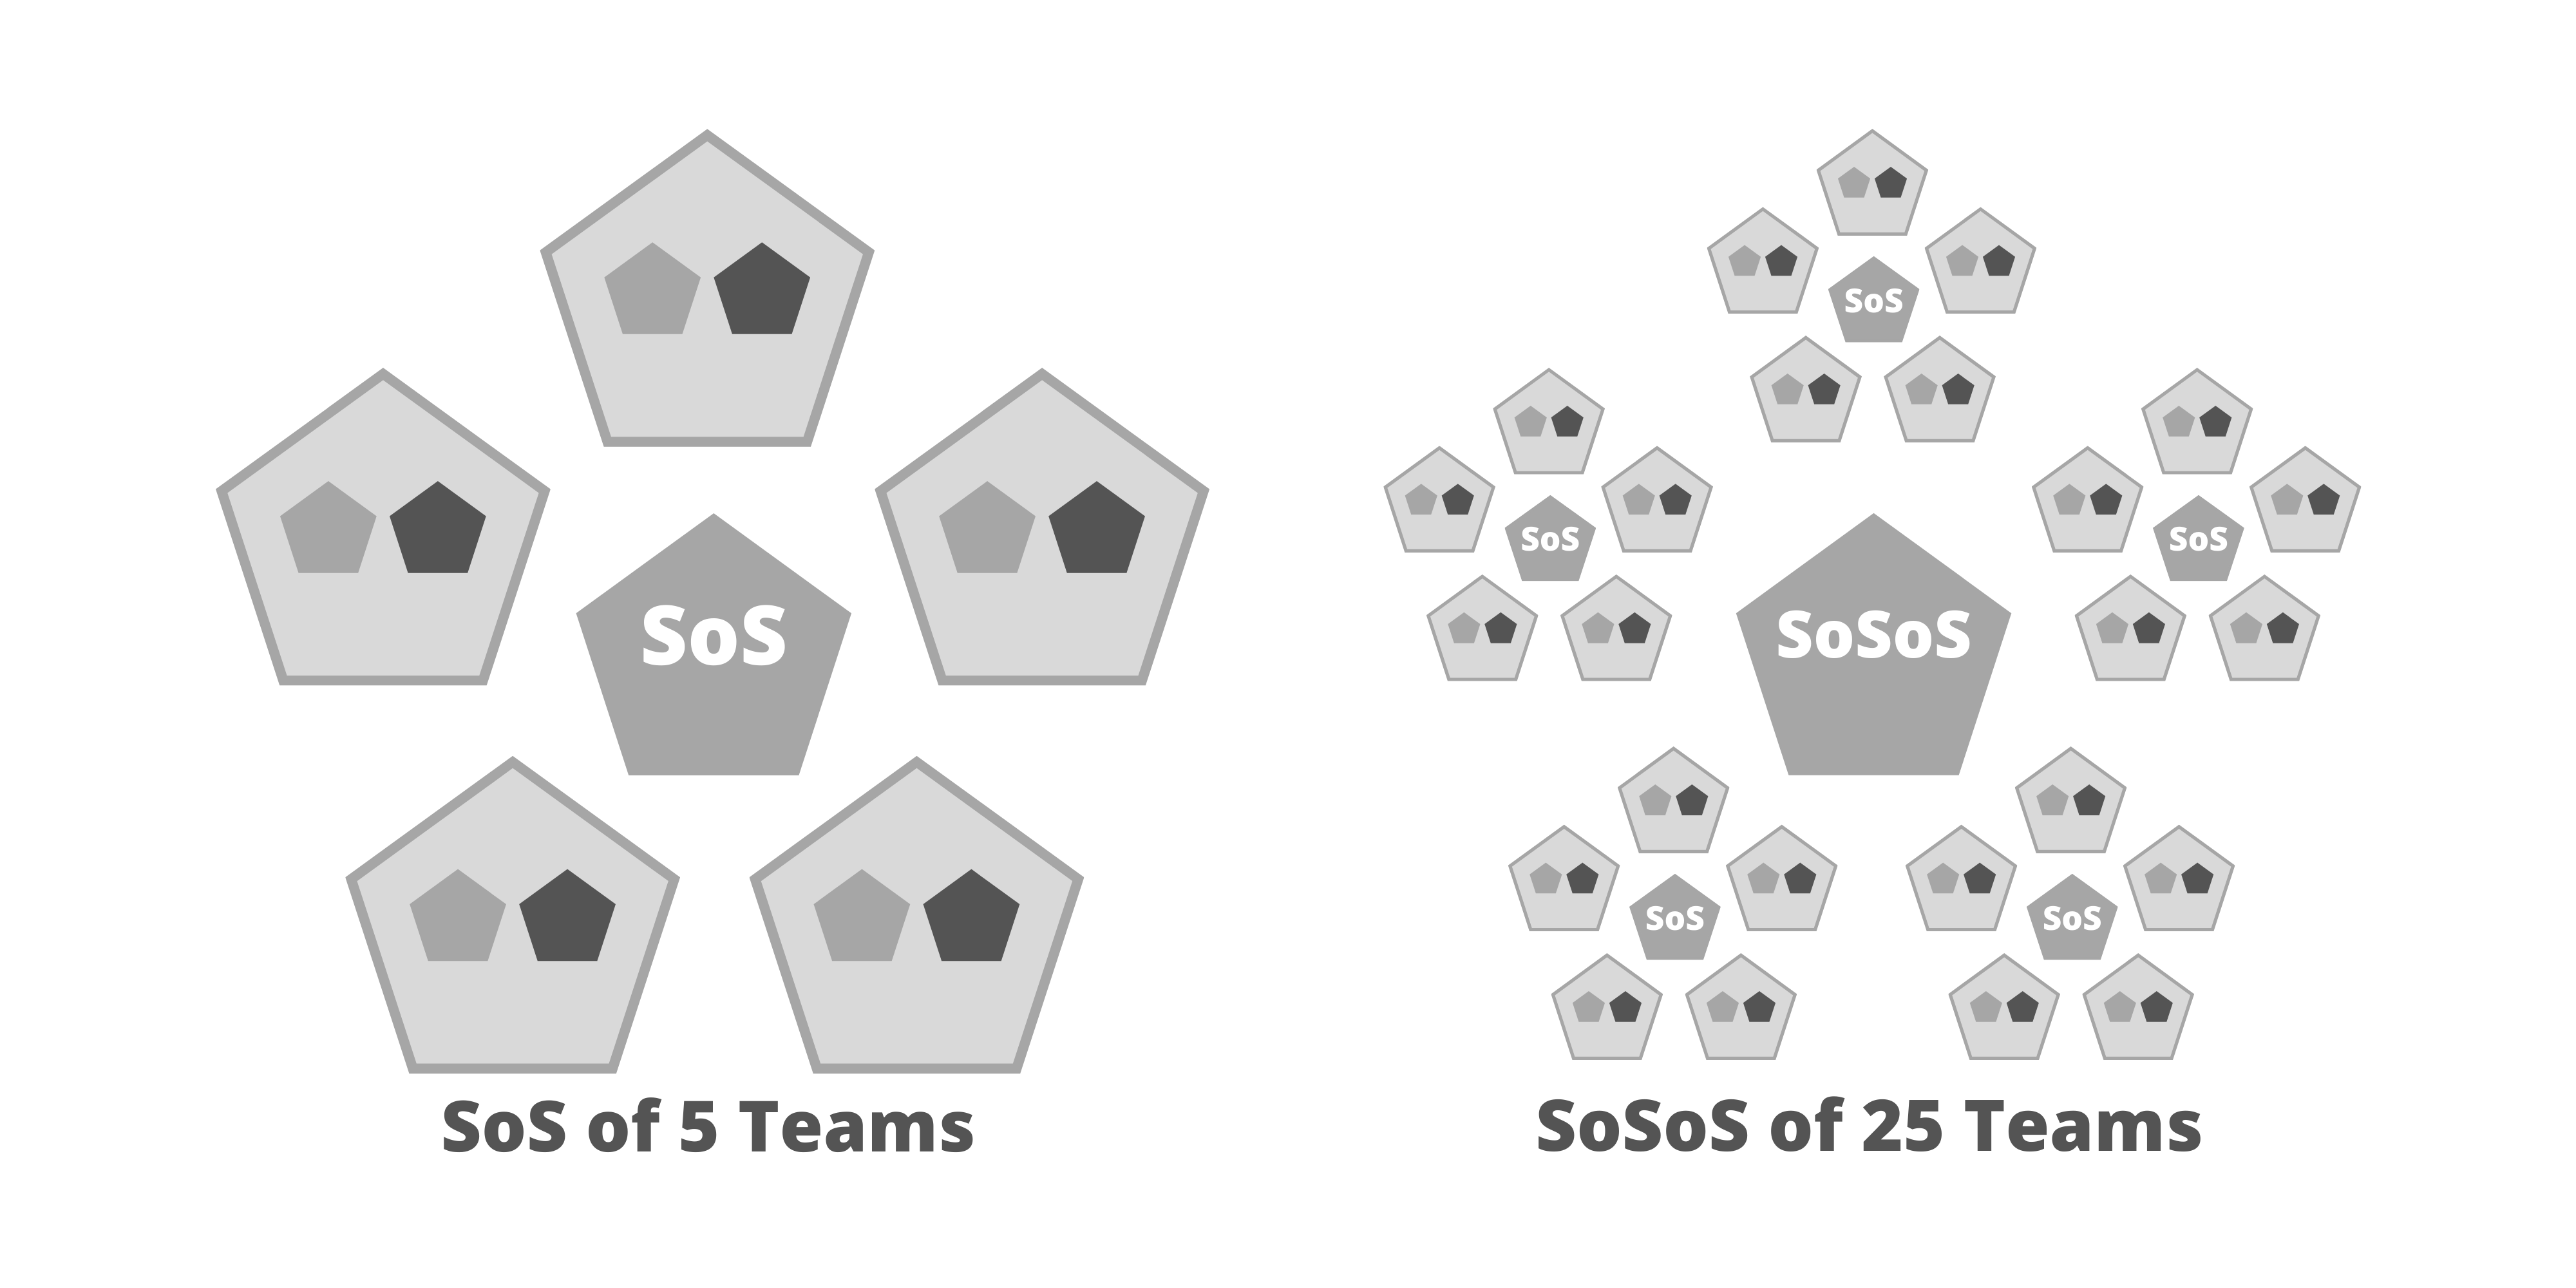
\includegraphics[scale=0.15]{2.png}
  
\end{figure}

\emph{NOTE: For simplicity, the numbers of teams and groupings in the
sample diagrams are symmetrical. They are meant to be examples only, as
each organizational diagram may differ greatly.}

\subsubsection{Scaling the Events and
Roles}\label{scaling-the-events-and-roles}

If a Scrum of Scrums (SoS) operates as a Scrum Team, then it needs to scale the Scrum Events and the teams' corresponding accountabilities. To coordinate the ``how'' in every Sprint, a SoS will need to hold scaled versions of the Daily Scrum and Sprint Retrospective. To coordinate the ``what'' in every Sprint, a SoS will need to hold scaled versions of Sprint Planning and a Sprint Review. As an ongoing practice, Backlog Refinement will also need to be done at scale.

The scaled versions of the Daily Scrum and Retrospective are facilitated by a Scrum Master for the group, called the Scrum of Scrums Master (SoSM). The scaled versions of the Sprint Review and Backlog Refinement are facilitated by a Product Owner Team guided by a Chief Product Owner (CPO). The scaled version of Sprint Planning is held with the Product Owner Team and the Scrum Masters. The Product Owner Team gains insight into what will be delivered in the current Sprint and the Scrum Masters gain insight into capacity and technical capabilities. The roles of Scrum of Scrums Master and Chief Product Owner scale into the leadership groups which then drive their corresponding cycles, satisfying the components of Scrum@Scale.


\subsubsection{Event: The Scaled Daily Scrum
(SDS)}\label{event-the-scaled-daily-scrum}


The main talking points of a Daily Scrum are the progress towards the Sprint Goal and impediments to meeting that commitment. In a scaled setting, the Scrum of Scrums needs to understand collective progress and be responsive to impediments raised by participating teams; therefore, at least one representative from each team attends a Scaled Daily Scrum (SDS). Any person or number of people from participating teams may attend as needed.

To optimize collaboration and performance, the Scaled Daily Scrum event mirrors the Daily Scrum, in that it:


\begin{itemize}
\itemsep1pt\parskip0pt\parsep0pt
\item
  Is time-boxed to 15 minutes or less
\item
  Must be attended by a representative of each team.
\item
  Is a forum to discuss how teams can work together more effectively,
  what has been done, what will be done, what is going wrong \& why, and
  what the group is going to do about it
\end{itemize}

Some examples of questions to be answered:

\begin{itemize}
\itemsep1pt\parskip0pt\parsep0pt
\item
  What impediments does a team have that will prevent them from accomplishing their Sprint Goal or that will impact the planned delivery?
\item
  Is a team doing anything that will prevent another team from accomplishing their Sprint Goal or that will impact their planned delivery?
\item
 Have any new dependencies between the teams or a way to resolve an existing dependency been discovered?
\end{itemize}

\subsubsection{Event: The Scaled
Retrospective}\label{event-the-scaled-retrospective}

Every Sprint, the Scrum of Scrums holds a scaled version of the Sprint Retrospective where the Scrum Masters of each team get together and discuss what experiments have been done to drive continuous improvement and their results. Additionally, they should discuss the next round of experiments and how successful improvements can be leveraged across the group of teams or beyond.

\subsection{The Scrum Master Cycle: Coordinating the
``How''}\label{the-scrum-master-cycle}

\subsubsection{Role: The Scrum of Scrums Master
(SoSM)}\label{role-the-scrum-of-scrums-master}

The Scrum Master of the Scrum of Scrums is called the Scrum of Scrums Master (SoSM). The Scrum of Scrums Master is accountable for ensuring the Scaled events take place, are productive, positive, and kept within the time-box. The Scrum of Scrums Master may be one of the team's Scrum Masters or a person specifically dedicated to this role. They are accountable for the release of the joint teams' efforts and continuously improving the effectiveness of the Scrum of Scrums. This includes greater team throughput, lower cost, and higher quality. In order to achieve these goals, they must:

\begin{itemize}
\itemsep1pt\parskip0pt\parsep0pt
\item
  Work closely with the Chief Product Owner to deliver a potentially
  releasable product increment at least every Sprint
\item
  Coordinate the teams' delivery with the Product Owners Team's release
  plans
\item
  Make impediments, process improvements, and progress visible to the
  organization
\item
  Facilitate the prioritization and removal of impediments, paying
  particular attention to cross-team dependencies
\end{itemize}

The Scrum of Scrums Master is a true leader who serves the teams and the organization by understanding cross-team dependencies, including those outside of the Scrum of Scrums and enabling cross-team coordination and communication. They are accountable for keeping the Chief Product Owner, stakeholders, and larger organization informed by radiating information about product development progress, impediments removal status, and other metrics. The Scrum of Scrums Master leads by example, mentoring others to increase the effectiveness and adoption of Scrum throughout the organization.

In the case where multiple Scrum of Scrums are grouped into a Scrum of Scrum of Scrums, then a Scrum of Scrum of Scrums Master (SoSoSM) is needed to coordinate from that wider perspective.


\subsubsection{The Hub of the SM Cycle: The Executive Action Team
(EAT)}\label{the-hub-of-the-sm-cycle}

The Executive Action Team (EAT) fulfills the Scrum Master accountabilities for an entire agile organization. This leadership team creates an agile ecosystem that allows the Reference Model to function optimally, by:

\begin{itemize}
\itemsep1pt\parskip0pt\parsep0pt
\item
  implementing the Scrum values
\item
  assuring that Scrum roles are created and supported
\item
  Scrum events are held and attended
\item
 Scrum Artifacts and their associated commitments are generated, made transparent, and updated throughout each Sprint.
\item
 formulating guidelines and procedures that act as a translation layer between the Reference model and any part of the organization that is not agile.
\end{itemize}

The Executive Action Team is accountable for removing impediments that cannot be removed by members of the Scrum of Scrums (or wider network). Therefore, it must be comprised of individuals who are empowered, politically and financially, to remove them. The function of the Executive Action Team is to coordinate multiple Scrums of Scrums (or wider networks) and to interface with any non-agile parts of the organization. As with any Scrum Team, it needs a Product Owner, a Scrum Master, and a transparent backlog.

\begin{figure}[H]
    \centering
    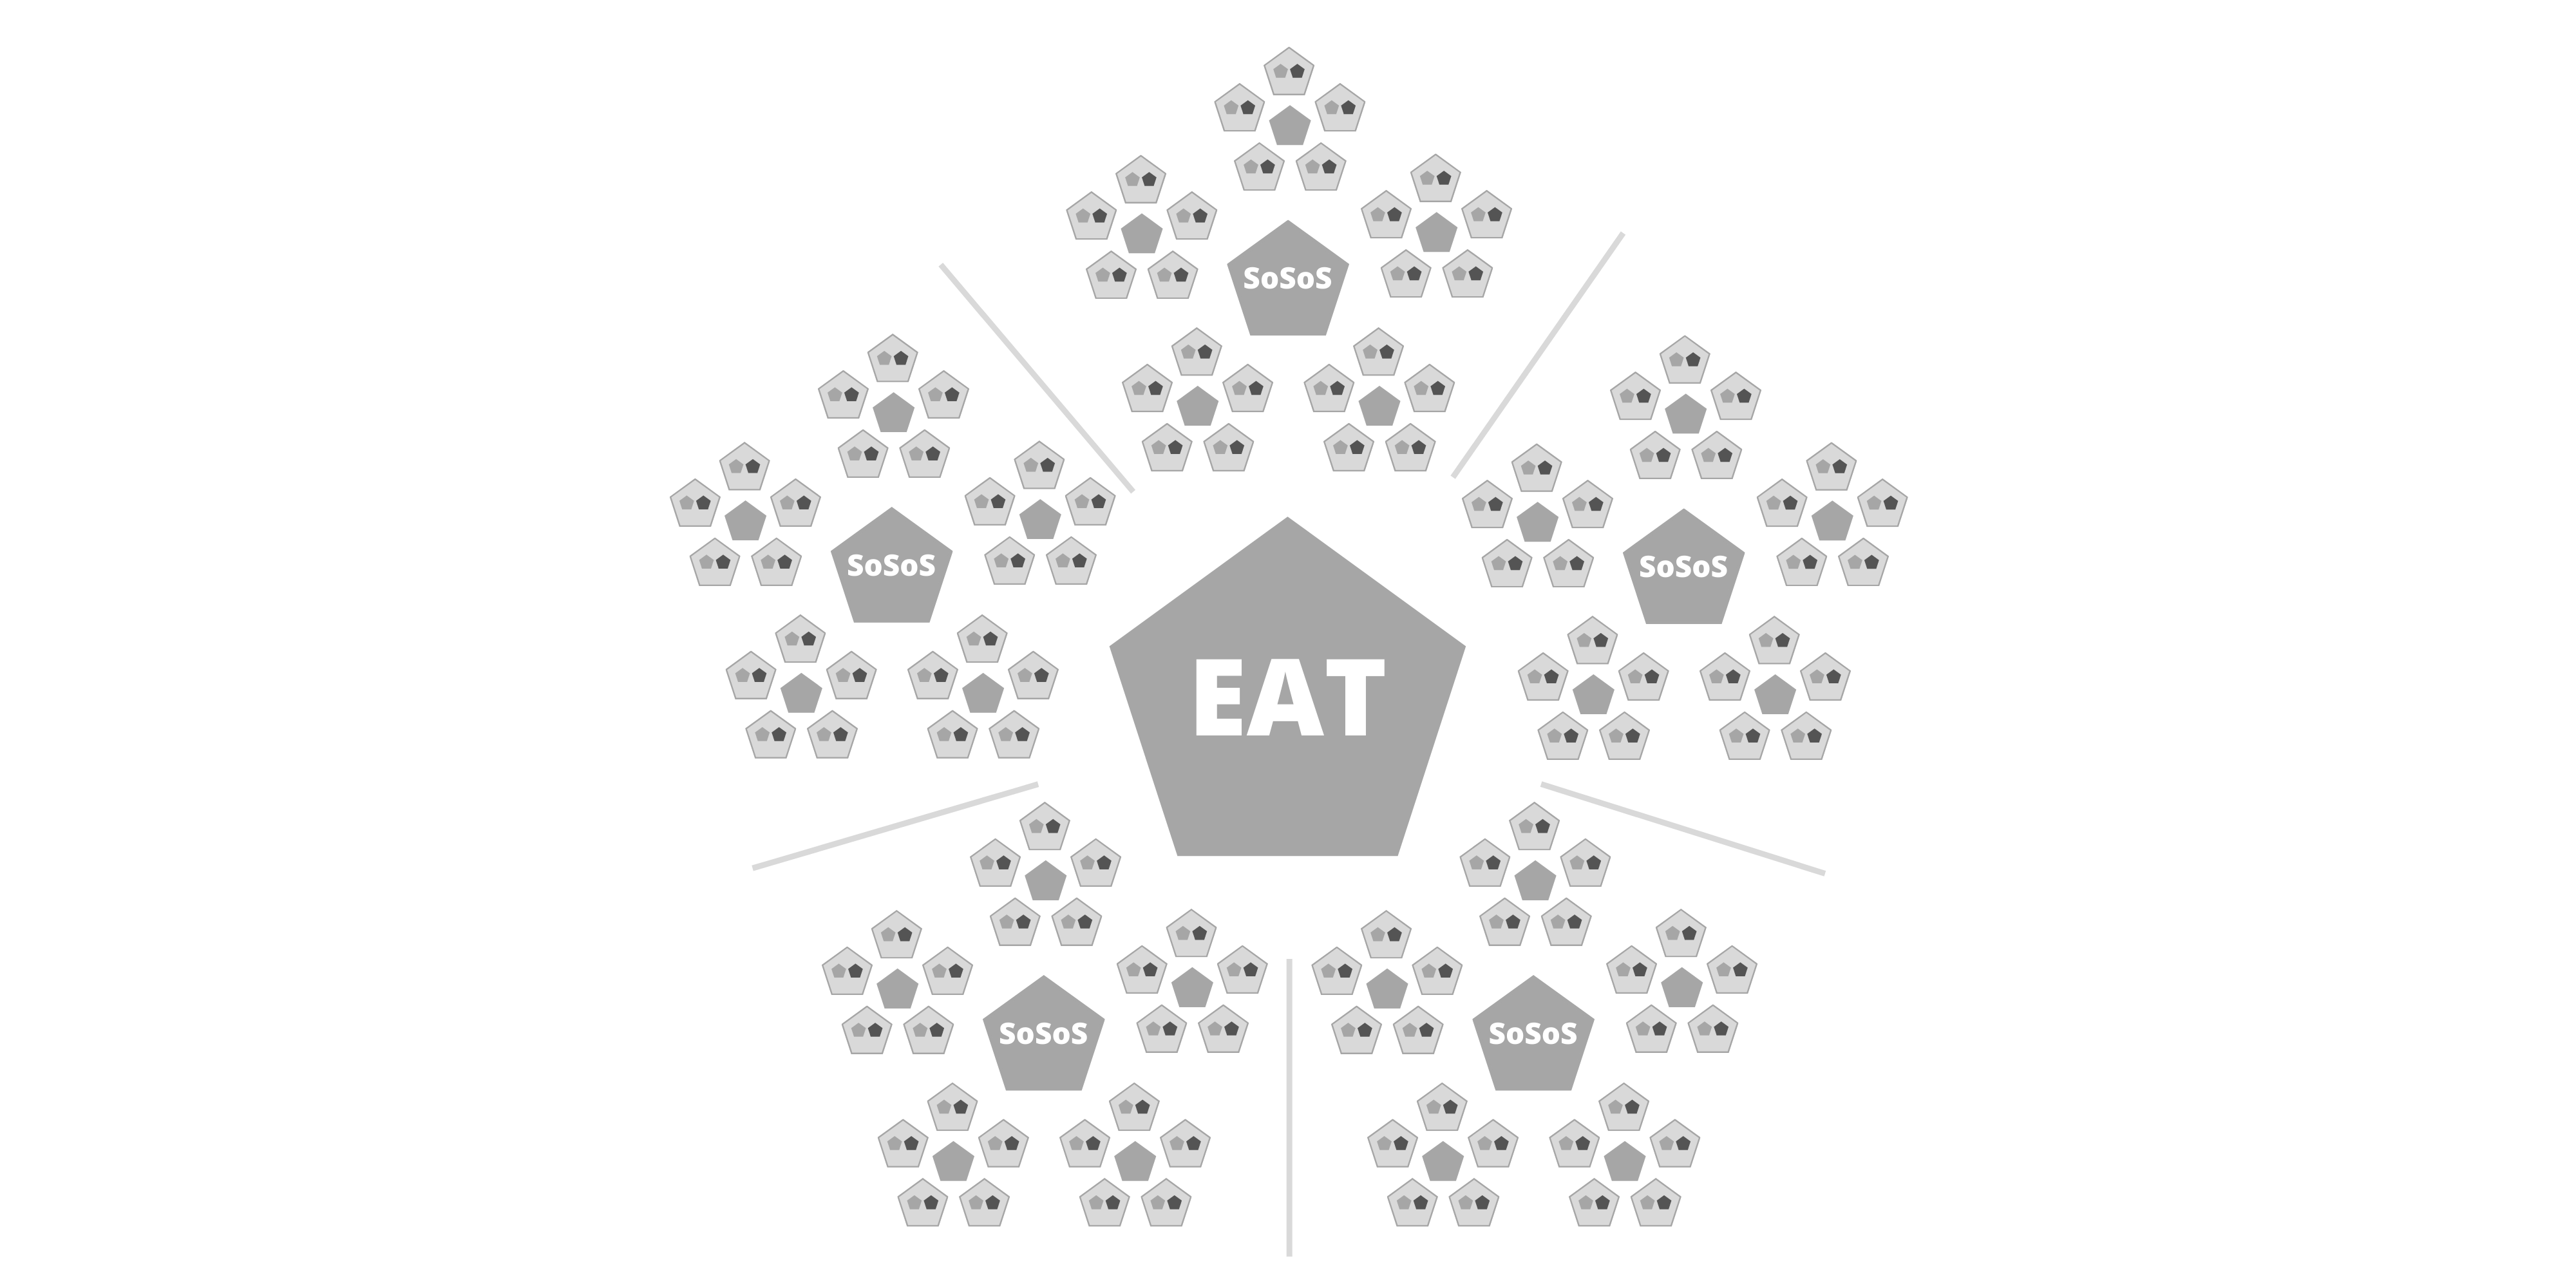
\includegraphics[scale=0.15]{3.png}
    
\end{figure}


\emph{Sample Diagram showing an EAT coordinating 5 groupings of 25
teams}

\subsubsection{EAT Backlog and
Responsibilities}\label{EAT-backlog-and-responsibilities}

The product of the Executive Action Team (EAT) is the creation of an Agile operating system for the organization. The EAT curates a Product Backlog consisting of initiatives for the ongoing transformation of the organization to achieve the goal of greater business agility. This backlog also includes process improvements which remove impediments and ones that need to be standardized.

The Executive Action Team's responsibilities include, but are not
limited to:

\begin{itemize}
\itemsep1pt\parskip0pt\parsep0pt
\item
  Creating an agile operating system for the Reference Model as it scales through an organization, including corporate operational rules, procedures, and guidelines to enable agility
\item
 Ensuring a Product Owner organization is created, funded, and supported
\item
  Measuring and improving the quality of Scrum in an organization
\item
  Building capability within an organization for business agility
\item
  Creating a center for continuous learning for Scrum professionals
\item
  Supporting the exploration of new ways of working
\end{itemize}

The function of the Executive Action Team is to see that this backlog is carried out. They may do this themselves or empower another group to do it. As the Executive Action Team is accountable for the quality of Scrum within the organization, the entire Scrum Master organization reports into them.

The Scrum Master organization (Scrum Masters, Scrum of Scrum Masters, and the Executive Action Team) work as a whole to implement the Scrum Master Cycle components. These unique components are:


\begin{itemize}
\itemsep1pt\parskip0pt\parsep0pt
\item
  Continuous Improvement and Impediment Removal
\item
  Cross-Team Coordination
\item
  Delivery
\end{itemize}

\subsubsection{Continuous Improvement and Impediment
Removal}\label{Continuous-improvement-and-impediment-removal}

Ideally, impediments should be removed as quickly as possible. This is critical to avoid scaling the impediments themselves, and because unresolved impediments may slow productivity. Therefore, the goals of Continuous Improvement and Impediment Removal are to:


\begin{itemize}
\itemsep1pt\parskip0pt\parsep0pt
\item
  identify impediments and reframe them as opportunities to improve
\item
  ensure transparency and visibility in the organization to effect
  change
\item
  maintain an effective environment for prioritizing and removing
  impediments
\item
  verify that improvements have positively impacted team and/or product
  metrics
\end{itemize}

\subsubsection{Cross-Team Coordination}\label{cross-team-coordination}

When multiple teams are needed for the creation of a shared product,
streamlined collaboration is required for success. Therefore, the goals
of Cross-Team Coordination are to:

\begin{itemize}
\itemsep1pt\parskip0pt\parsep0pt
\item
  sync up similar processes across multiple related teams
\item
  mitigate cross-team dependencies to ensure they do not become
  impediments
\item
  maintain alignment of team norms and guidelines for consistent output
\end{itemize}

\subsubsection{Delivery}\label{Delivery}

Since the goal of the Scrum of Scrums is to function as a single unit and release together, how the product is delivered falls under their scope as a group. The Product Owner Team determines both the content of the release and the optimal time to deliver the increment to customers.  Therefore, the goals of Delivery for the Scrum of Scrums are to:

\begin{itemize}
\itemsep1pt\parskip0pt\parsep0pt
\item
  deliver a consistent flow of valuable finished product to customers
\item
  integrate the work of different teams into one seamless product
\item
  ensure a high-quality customer experience
\end{itemize}

\subsection{The Product Owner Cycle: Coordinating the
``What''}\label{The-product-owner-cycle}

\subsubsection{Scaling the Product Owner - The Product Owner
Cycle}\label{Scaling-the-product-owner}

For each Scrum of Scrums, there is a shared common backlog that feeds the network of teams. It requires a Product Owner Team (PO Team), including a Chief Product Owner, who is accountable as the Product Owner for the group of teams. The PO Team's main focus is ensuring that the individual teams' priorities follow along a single path. This allows them to coordinate their individual team's backlogs and build alignment with stakeholders and customer needs.


Each team's Product Owner is accountable for the composition and prioritization of their team's Sprint backlog and may pull items from the common backlog or generate independent backlog items at their discretion as needed to meet business objectives.

The main functions of the Product Owner Team are to:

\begin{itemize}
\itemsep1pt\parskip0pt\parsep0pt
\item
  communicate the overarching vision for the product \& make it visible
  to everyone in the organization
\item
  build alignment with key stakeholders to secure support for backlog
  implementation
\item
  generate a single, prioritized backlog; ensuring that duplication of
  work is avoided
\item
  work with the Scrum of Scrums Master to create a minimally uniform
  ``Definition of Done'' that applies to all team
\item
  eliminate dependencies raised by the teams
\item
  generate a coordinated Roadmap and Release Plan
\item
  monitor metrics that give insight into the product and the market
\end{itemize}

\subsubsection{Role: The Chief Product Owner
(CPO)}\label{role-the-chief-product-owner}

The Chief Product Owner coordinates priorities with the Product Owner Team. Together they align backlog priorities with stakeholder and customer needs. The CPO may be an individual team Product Owner who plays this role as well, or they may be a person specifically dedicated to it. Their main responsibilities are the same as a regular Product Owner's now scaled:

\begin{itemize}
\itemsep1pt\parskip0pt\parsep0pt
\item
  Setting a strategic vision for the whole product
\item
  Creating a single, prioritized backlog to be delivered by all of the
  teams
\item
  Decide which metrics the Product Owner Team will monitor
\item
  Assess customer product feedback and adjust the common backlog
  accordingly
\item
  Facilitate the MetaScrum event (see below)
\end{itemize}

The Chief Product Owner is accountable along with their associated Scrum
of Scrums Masters for the efficient delivery of product increments
according to the Release Plan.

\subsubsection{Scaling the Product Owner
Team}\label{scaling-the-product-owner-team}

Having Product Owner Teams enables a network design of Product Owners which scales along with their associated Scrum of Scrums. There is no specific term associated with these expanded units, nor do the Chief Product Owners of them have specific expanded titles. Each organization is encouraged to develop their own.

\subsubsection{The Hub of the PO Cycle: The Executive MetaScrum
(EMS)}\label{the-hub-of-the-po-cycle}

To fulfill the Product Owner role for the entire agile organization, the
Chief Product Owners meet with executives and key stakeholders at an
Executive MetaScrum event. This event is derived from the MetaScrum
pattern\textsuperscript{\hyperref[citation5]{5}}. It is \emph{the forum}
for Leadership and other stakeholders to express their preferences to
the PO Team, negotiate priorities, alter budgets, or realign teams to
maximize the delivery of value. At no other time during the Sprint
should these decisions be made.

At the Executive MetaScrum a dynamic group of leaders sets the
organizational vision and the strategic priorities, aligning all of the
teams around common goals.~ In order to be effective, the Chief Product
Owner facilitates and each team's Product Owner (or a proxy) must
attend. This event occurs as often as needed- at least once per Sprint-
to ensure an aligned backlog within the Scrum of Scrums.~ Optimally,
this group of leaders operates as a scrum team.

In the case of larger implementations where there are multiple Scrum of
Scrums, there may be multiple MetaScrums which have their strategic
backlog created and prioritized at an Executive MetaScrum.

\subsubsection{Coordinating the ``What'' - The Product Owner
Cycle}\label{coordinating-the-what}

The Product Owner organization (the Product Owners, the Chief Product
Owners, and the Executive MetaScrum) work as a whole to satisfy the
unique components of the Product Owner Cycle:

\begin{itemize}
\itemsep1pt\parskip0pt\parsep0pt
\item
  Strategic Vision
\item
  Backlog Prioritization
\item
  Backlog Decomposition \& Refinement
\item
  Release Planning
\end{itemize}

\subsubsection{Strategic Vision}\label{strategic-vision}

A compelling vision attracts both customers and great employees.
Therefore, formulate a Strategic Vision to be communicated, both
externally and internally, with the goals of:

\begin{itemize}
\itemsep1pt\parskip0pt\parsep0pt
\item
  aligning the entire organization along a shared path forward
\item
  compellingly articulating why the organization and its products exist
\item
 clarity allowing for the creation of concrete Product Goals
\item
describing what the organization will do to leverage key assets
\item
being able to respond to rapidly changing market conditions
\end{itemize}

\subsubsection{Backlog Prioritization}\label{backlog-prioritization}

Proper backlog prioritization is essential for teams to work in a coordinated manner to optimize value delivery. Competition between priorities creates waste because it pulls teams in opposing directions. The goals of Backlog Prioritization are to:

\begin{itemize}
\itemsep1pt\parskip0pt\parsep0pt
\item
  identify a clear ordering for products, capabilities, and services to
  be delivered
\item
  reflect value creation, risk mitigation, and internal dependencies in
  ordering of the backlog
\item
  prioritize the high-level initiatives across the entire agile
  organization prior to Backlog Decomposition and Refinement
\end{itemize}

\subsubsection{Backlog Decomposition and
Refinement}\label{backlog-decomposition-and-refinement}

A Chief Product Owner's backlog contains items which are larger in scope than an individual team's backlog. To pull prioritized items into individual teams, they may need to be broken down and understood better. The goals of Backlog Decomposition and Refinement are to:

\begin{itemize}
\itemsep1pt\parskip0pt\parsep0pt
\item
  identify the complex products, projects, and associated Product Goals which will make the vision a reality
\item
  break those complex products and projects into independent elements
\item
  ensure all backlog items can be refined further by the teams into items they can complete in one Sprint
\end{itemize}

\subsubsection{Release Planning}\label{Release-planning}

Release Planning may encompass one or many releases of the product to a customer. It is a longer-term planning horizon than a single Sprint. The goals of Release Planning are to:

\begin{itemize}
\itemsep1pt\parskip0pt\parsep0pt
\item
  forecast the delivery timeline of key Product Increments and
  capabilities.
\item
  communicate delivery expectations to stakeholders.
\item
  communicate the financial impact of the delivery schedule.
\end{itemize}

\subsection{Connecting the Product Owner and Scrum Master
Cycles}\label{Connecting-the-product-owner-and-scrum-master-cycles}

The cycles first intersect at the Team Process component. From that point, the accountability for the ``what'' and ``how'' separate until done product gets delivered. The cycles connect again within the Feedback component where customer response to the product is interpreted. This requires Metrics in order to make empirical decisions about adapting for the next delivery cycle. The Product Owner and Scrum Master organizations work together to fulfill the requirements of these components.

\subsubsection{Product Feedback and Release
Feedback}\label{product-feedback-and-release-feedback}

Product feedback is interpreted by the Product Owner organization to drive continuous improvement of the product through updating the Product Backlog(s). Release feedback is interpreted by the Scrum Master organization to drive continuous improvement of the Delivery mechanisms. The goals of obtaining and analyzing Feedback are to:

\begin{itemize}
\itemsep1pt\parskip0pt\parsep0pt
\item
  validate assumptions
\item
  understand how customers use and interact with the product
\item
  capture new ideas and emerging requirements for new functionality
\end{itemize}

\subsubsection{Metrics and Transparency}\label{Metrics-and-transparency}

Metrics may be unique to both specific organizations as well as to specific functions within those organizations. Scrum@Scale does not require any specific set of metrics, but it does suggest that at a bare minimum, the organization should measure:

\begin{itemize}
\itemsep1pt\parskip0pt\parsep0pt
\item
  Productivity - e.g. change in amount of working product delivered per
  Sprint
\item
  Value Delivery - e.g. business value per unit of team effort
\item
  Quality - e.g. defect rate or service down-time
\item
  Sustainability - e.g. team happiness
\end{itemize}

Radical transparency is essential for Scrum to function optimally, giving the organization the ability to honestly assess its progress and to inspect and adapt its products and processes.

The goals of having Metrics and Transparency are to:

\begin{itemize}
\itemsep1pt\parskip0pt\parsep0pt
\item
  provide the appropriate context with which to make data-driven
  decisions
\item
  reduce decision latency
\item
  streamline the work required by teams, stakeholders or leadership
\end{itemize}

\subsubsection{Some Notes on Organizational
Design}\label{some-notes-on-organizational-design}

The goal of organizational design with Scrum@Scale is to allow it to be component-based, just like the framework itself. This permits for rebalancing or refactoring of teams in response to the market.

Sample diagrams:
\begin{figure}[H]
    \centering
    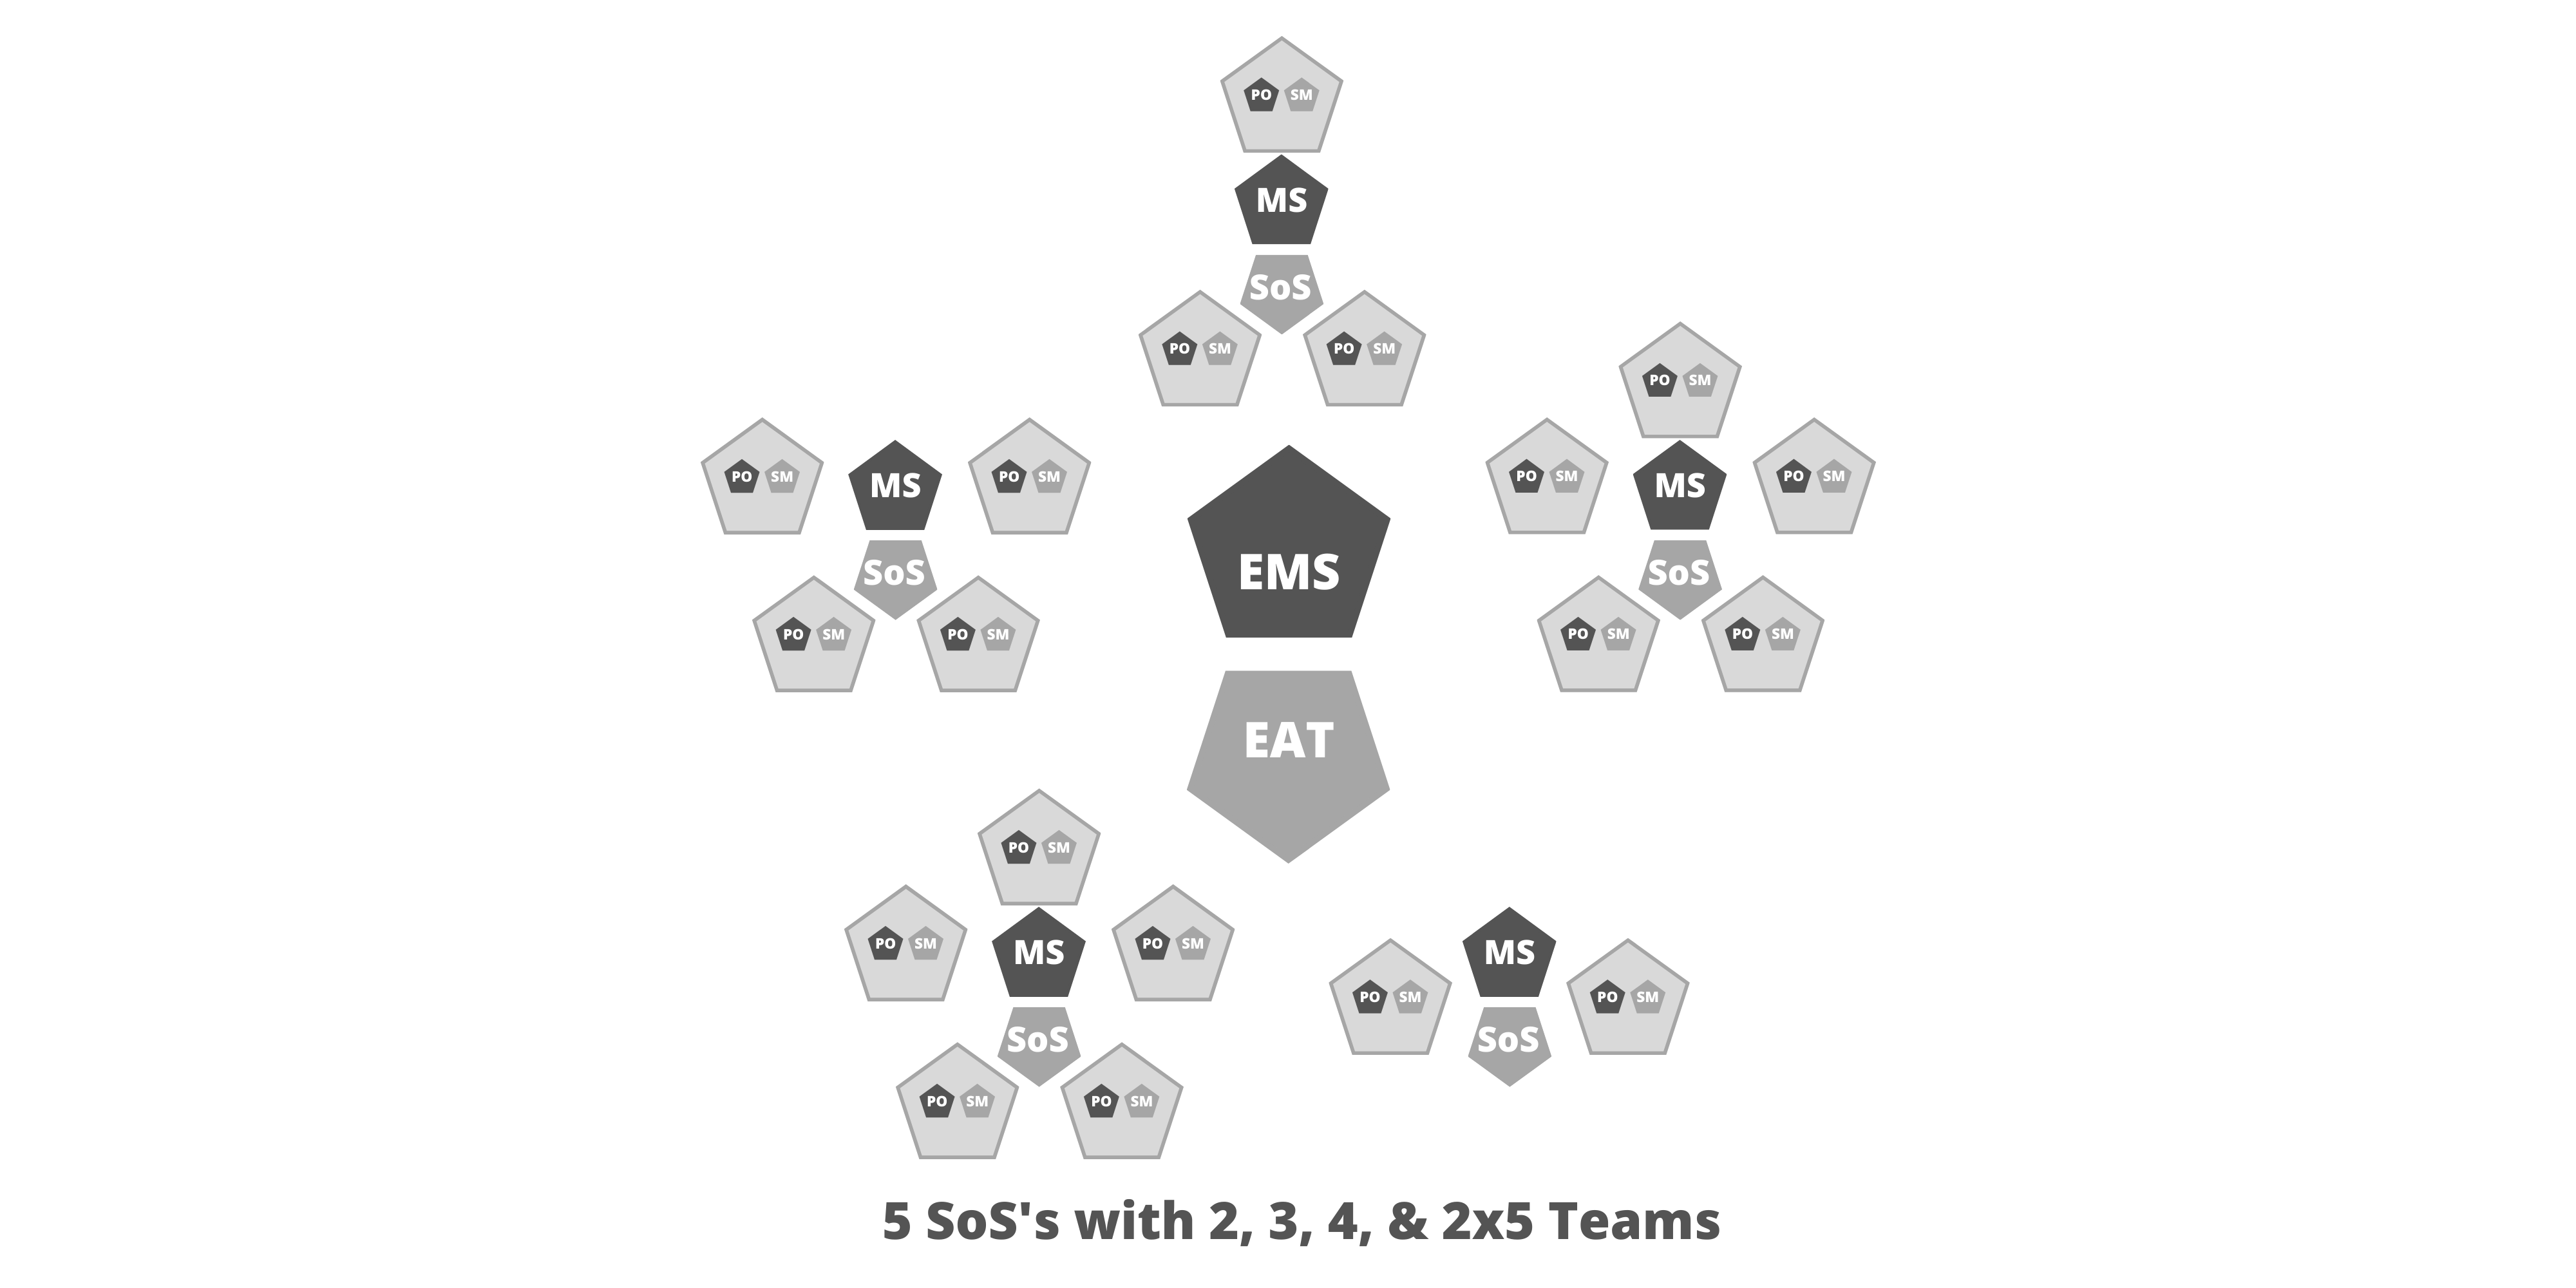
\includegraphics[scale=0.15]{4.png}
\end{figure}


\begin{figure}[H]
    \centering
    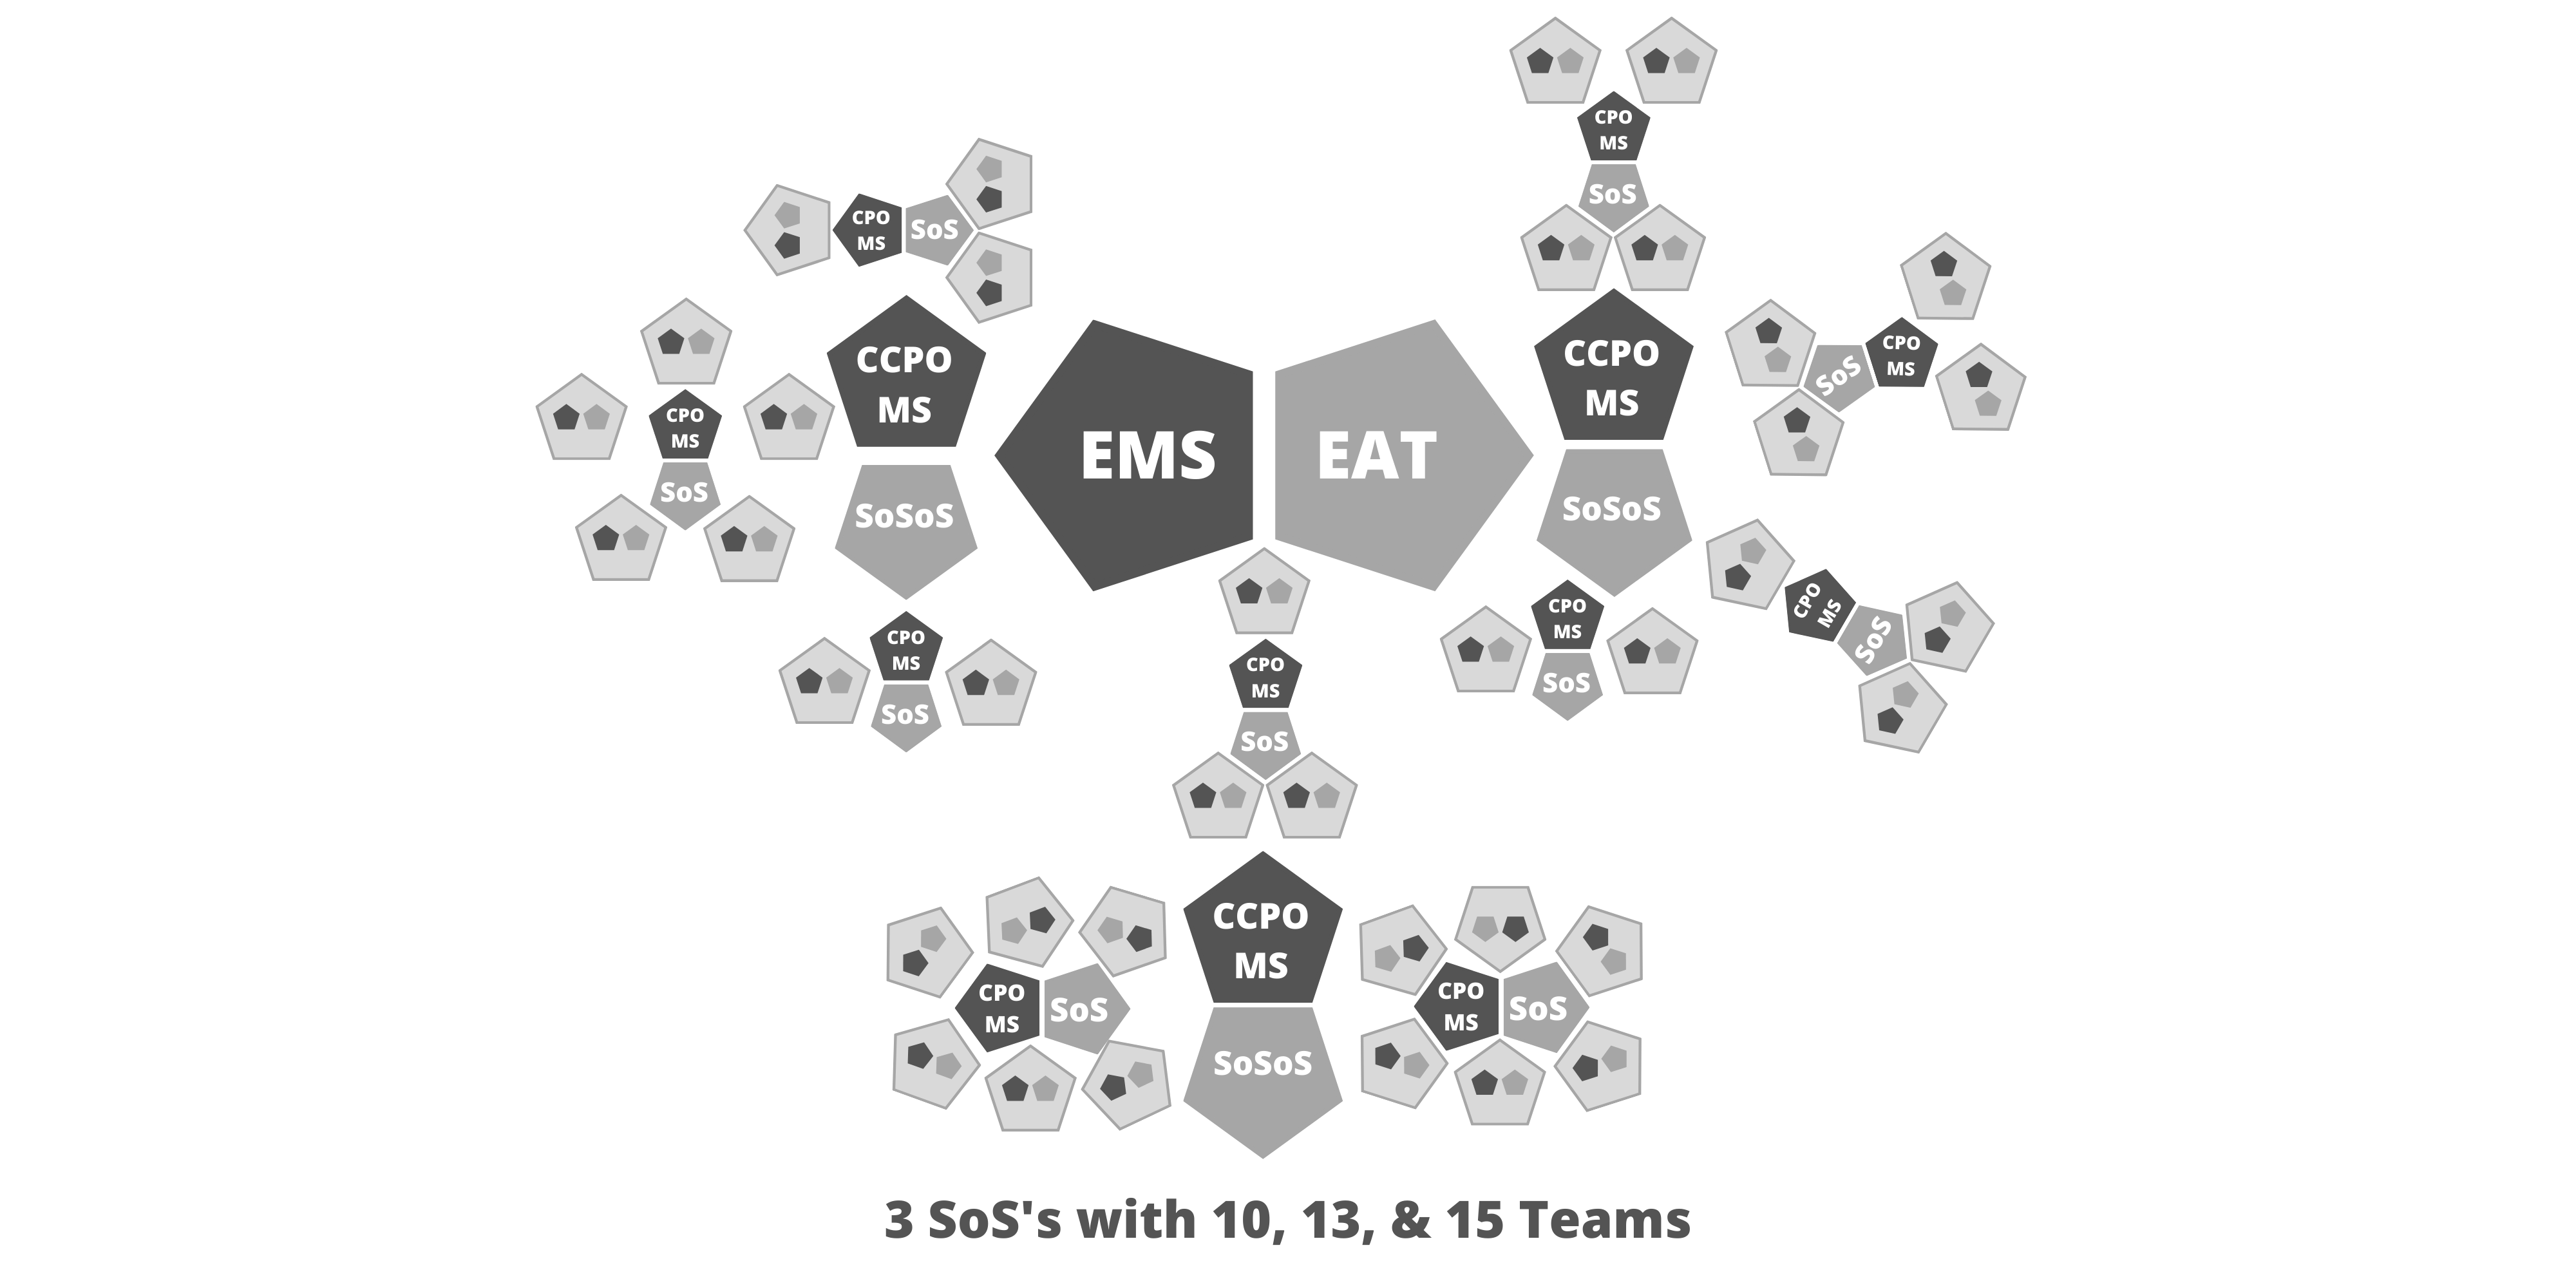
\includegraphics[scale=0.15]{5.png}
\end{figure}

Customer Relations, Legal / Compliance, and People Operations are included here since they are necessary parts of organizations and will exist as independent Scrum Teams on their own, upon which all other teams may rely.

A final note on the representation of the Executive Action Team and the Executive MetaScrum: In this diagram, they are shown as overlapping since some members sit on both of the teams. In very small organizations or implementations, the Executive Action Team and the Executive MetaScrum may consist entirely of the same team members.

\begin{figure}[H]
    \centering
    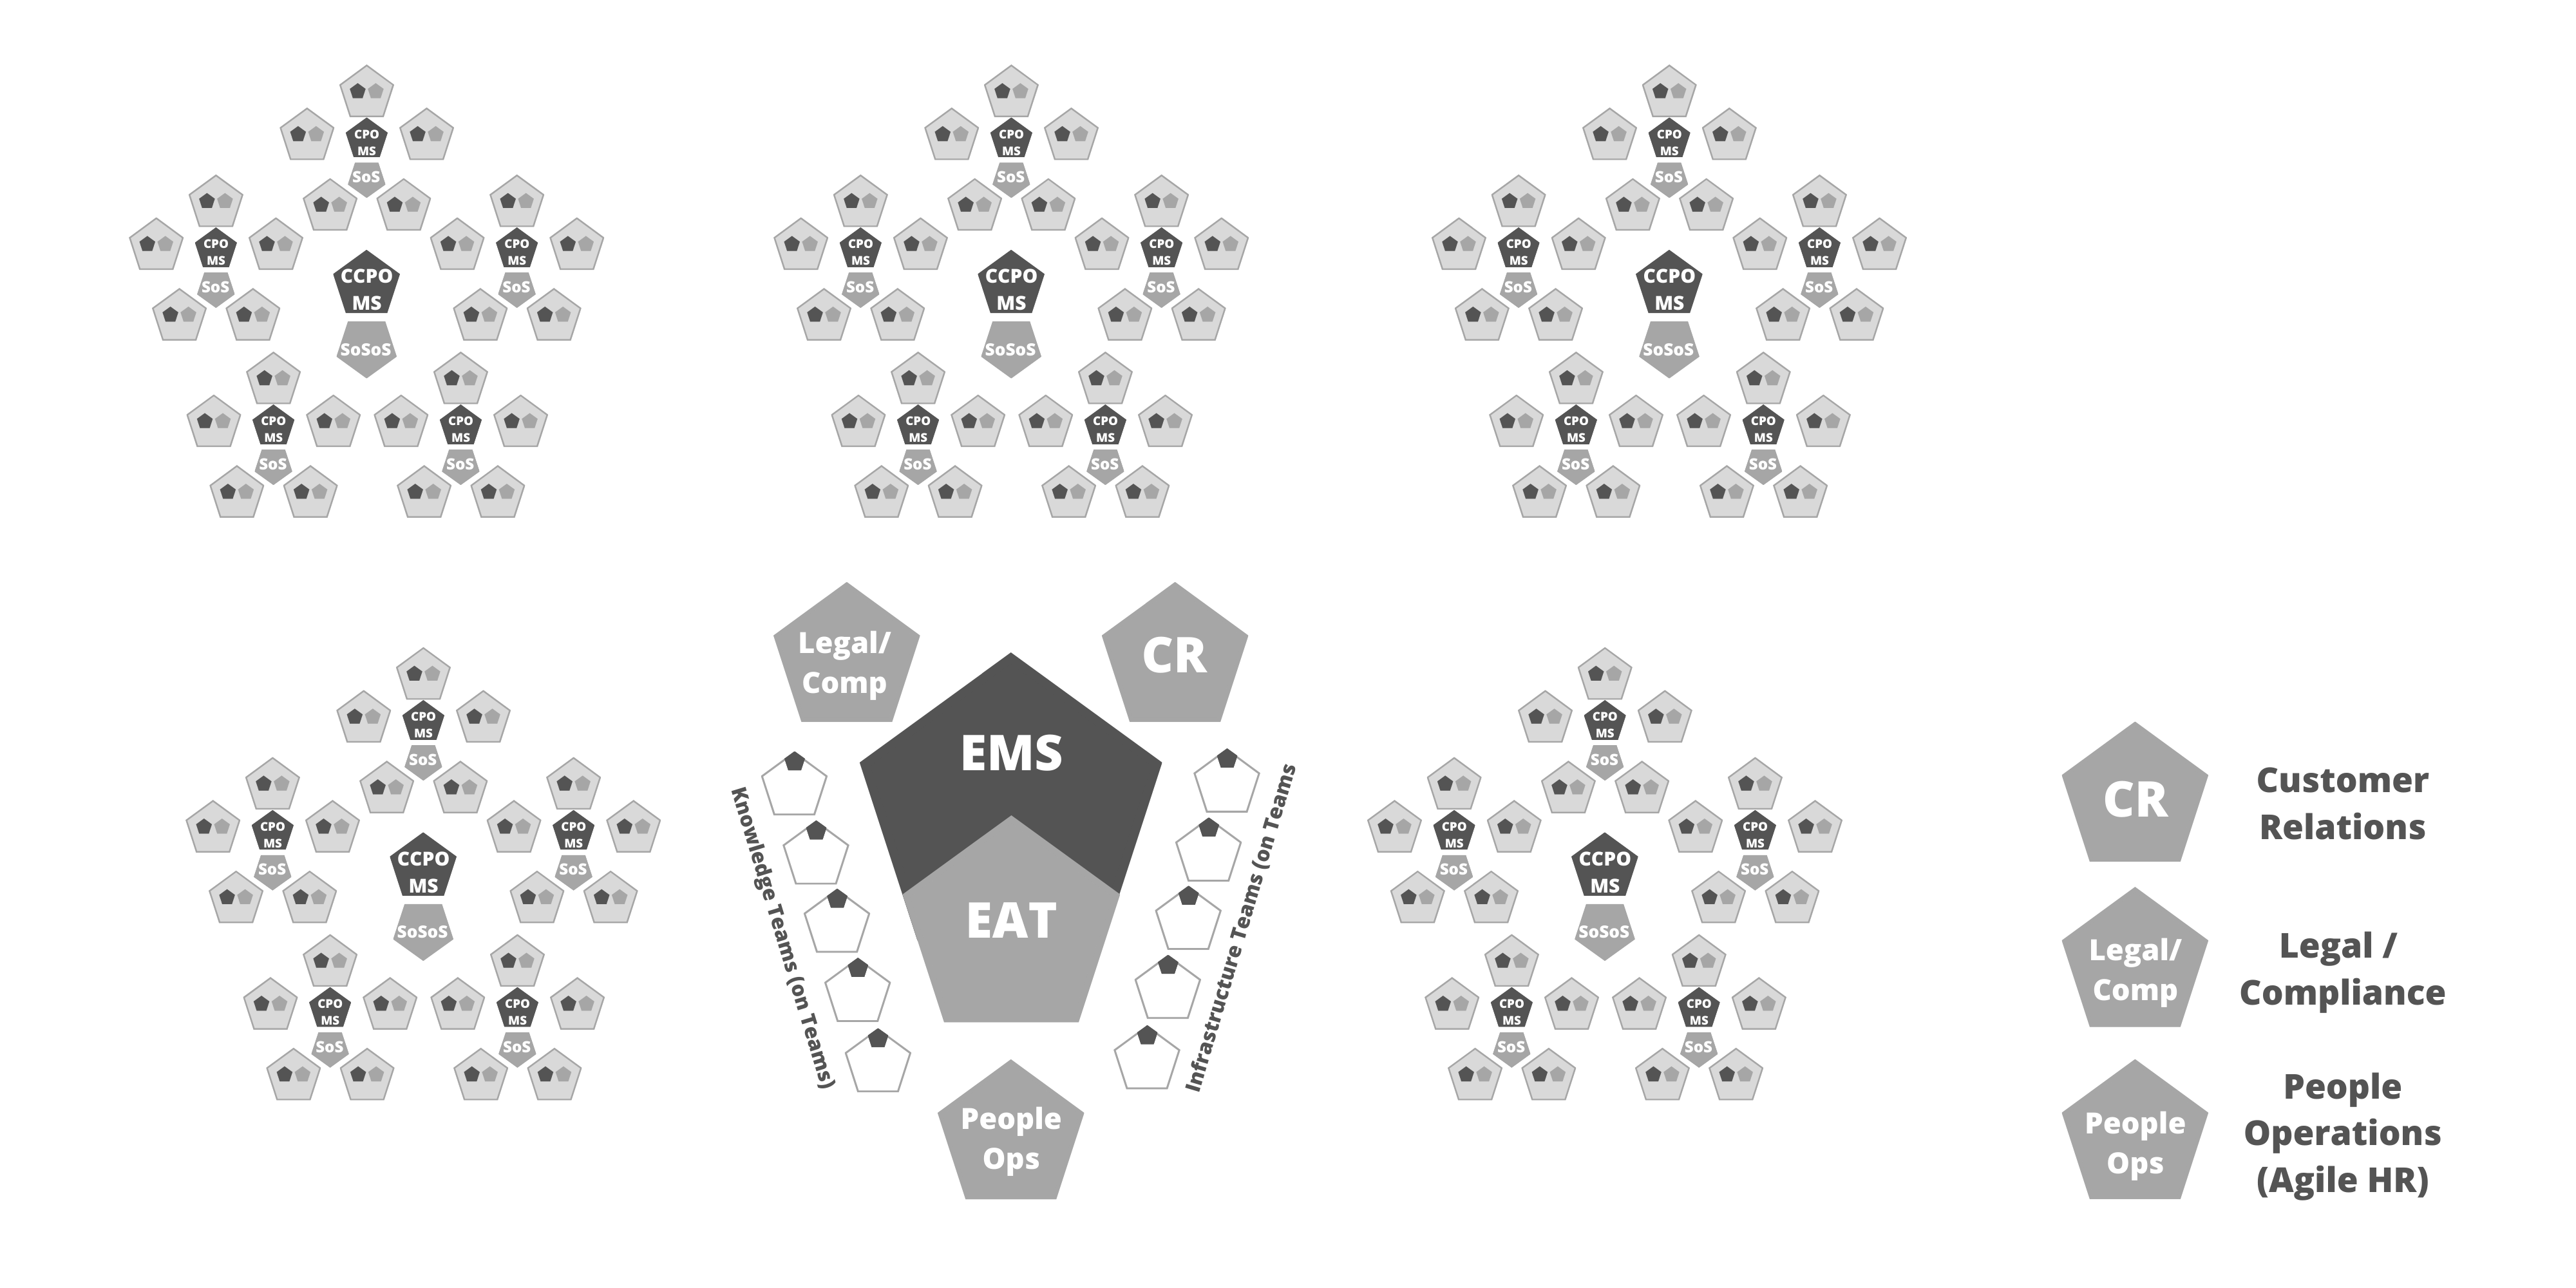
\includegraphics[scale=0.15]{6.png}
\end{figure}


\emph{In this organizational diagram, the Knowledge and Infrastructure Teams represent virtual teams of specialists of which there are too few to staff each team. If they act as shared-services team, they coordinate with the Scrum Teams as a group, where requests flow through a Product Owner for each specialty who converts them into a transparent prioritized backlog. An important note is that these teams are NOT silos of individuals who sit together (this is why they are represented as hollow pentagons); their team members sit on the actual Scrum Teams, but they make up this virtual Scrum of their own for the purpose of backlog dissemination and process improvement.}



\subsection{End Note}\label{End-Note}

Scrum@Scale is designed to scale productivity, to get an entire
organization delivering twice the value at half the cost. Implementing a
streamlined workflow at a sustainable pace with better decision making
improves the work environment, increases business agility, and generates
higher returns to all stakeholders.

Scrum@Scale is designed to saturate an organization with Scrum. Well
implemented Scrum can run an entire organization with Scrum@Scale as the
operating system.

\subsection{Acknowledgements}\label{Acknowledgements}

\subsubsection{History}\label{History}

Dr. Jeff Sutherland developed Scrum@Scale based on the fundamental principles behind Scrum, Complex Adaptive Systems theory, game theory, and his work in biology. The original version of this guide was created by collaboration with Jessica Larsen, Avi Schneier, and Alex Sutherland. Subsequent editions have been refined with the input of many experienced Scrum practitioners based on the results of their field work.

\subsubsection{People and Organizations}\label{People-and-Organizations}

We acknowledge IDX for the creation of the Scrum of Scrums which first
allowed Scrum to scale to hundreds of
teams\textsuperscript{\hyperref[citation6]{6}}, PatientKeeper for the
creation of the MetaScrum\textsuperscript{\hyperref[citation7]{7}},
which enabled rapid deployment of innovative product, and OpenView
Venture Partners for scaling Scrum to the entire
organization\textsuperscript{\hyperref[citation8]{8}}. We value input
from Intel, who taught us ``nothing scales except a scale-free
architecture'', and SAP, with the largest Scrum team product
organization, who taught us management involvement in the MetaScrum is
essential to get more than 2,000 Scrum Teams to work together.

The agile coaches and trainers implementing these concepts at Amazon, GE, 3M, Toyota, Spotify, Maersk, Comcast, AT\&T and many other companies have been helpful in testing these concepts across a wide range of businesses across different domains

~
\pagebreak
\begin{center}\rule{3in}{0.4pt}\end{center}

\begin{enumerate}
\itemsep1pt\parskip0pt\parsep0pt
\item
  ``Business agility.'' Wikipedia, Last modified 27 February
  2020.
  \newline ~\href{https://en.wikipedia.org/wiki/Business_agility}{https://en.wikipedia.org/wiki/Business\_agility}.
\item
  Johnson, Jim. New CHAOS Report. The Standish Group. 2018.
\item
  Ogunnaike, Babatunde A. and Ray, W. Harmon. Process Dynamics, Modeling
  and Control. Oxford University Press. 1994.
\item
  Hackman, J Richard. Leading Teams: Setting the Stage for Great
  Performances. Harvard Business Press. 2002.
\item
  Sutherland, Jeff, Coplien, James O., and The Scrum Patterns Group. A
  Scrum Book: The Spirit of the Game. Pragmatic Bookshelf. 2019.
\item
  Sutherland, Jeff. ``Inventing and Reinventing SCRUM in five
  Companies.'' Sur le site officiel de l'alliance agile. 2001.
\item
  Sutherland, Jeff. ``Future of Scrum: Parallel Pipelining of Sprints in
  Complex Projects.'' Proceedings of the Agile Development Conference.
  IEEE Computer Society 90-102. 2005.
\item
  Sutherland, Jeff and Altman, Igor. ``Take No Prisoners: How a Venture
  Capital Group Does Scrum.'' Agile Conference, 2009. AGILE'09, IEEE
  350-355. 2009.
\end{enumerate}

\end{document}
